\documentclass{article}
\usepackage{amsmath}
\usepackage{graphicx}
\usepackage{fancyhdr}
\usepackage[spanish]{babel}
\usepackage[utf8]{inputenc}

\parindent 0em
\parskip 2ex
\pagestyle{fancy}
\setlength{\textfloatsep}{5pt}

\begin{document}

\begin{titlepage}
\newcommand{\HRule}{\rule{\linewidth}{0.5mm}}

\center
\textsc{\LARGE ITESO, Universidad Jesuita De Guadalajara}\\[2cm]
\textsc{\Large INGENIERÍA FINANCIERA}\\[1cm]
\textsc{\large Innovación y Gestión De Proyectos}\\[1cm]
\HRule \\[2cm]
{ \huge \bfseries Accidentes viales en la ZMG}\\[2cm] 
\HRule \\[2cm]
\begin{minipage}{0.4\textwidth}
\begin{flushleft} \large


\emph{Autores:}\\
Rodrigo \textsc{Hernández Mota}\\
Ana Goretti \textsc{Chávez Flores}\\
Alicia Karime \textsc{González Beltrán}\\
José Felipe \textsc{}{Sanchez Andaluz}
\end{flushleft}
\end{minipage}
~
\begin{minipage}{0.4\textwidth}
\begin{flushright} \large
\emph{Supervisor:} \\
Mtra. Mireya \textsc{Pasillas Torres}
\end{flushright}
\end{minipage}\\[2cm]

{\large \today}\\[1cm]

\vfill
 
\end{titlepage}
\tableofcontents
\newpage

\section{Introducción}\label{sec:into}
[agregar contenido]

\section{Diagnóstico}\label{sec:diagnostic}

[agregar contenido]

	\begin{figure}[H]\centering
	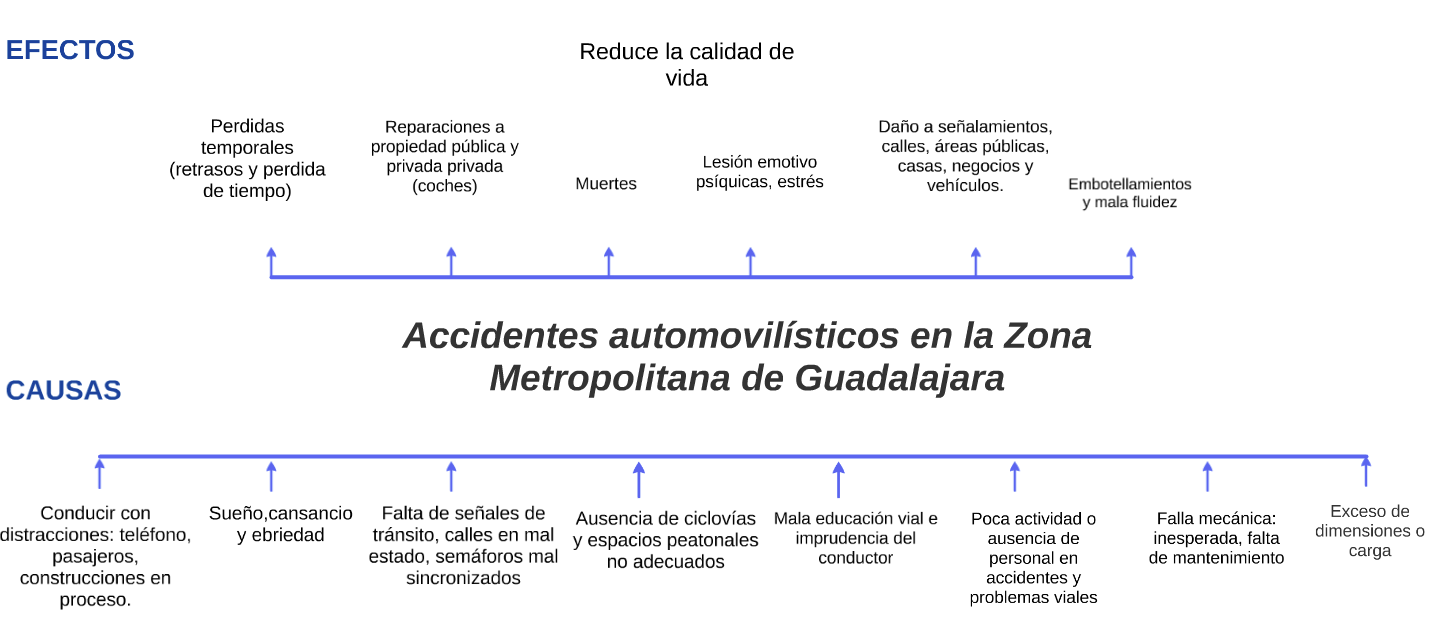
\includegraphics[width=0.8\textwidth]{resources/img/arbol_de_problemas.png}
	\caption{\label{} Árbol de problemas}
    \end{figure}

[agregar contenido]

\section{Objetivos del proyecto}\label{sec:objs}
[agregar contenido]

\subsection{Objetivos general}\label{subsec:general-objs}
[agregar contenido]

\subsection{Objetivos específico}\label{subsec:specific-objs}
[agregar contenido]

\section{Análisis de los participantes}\label{sec:participants}
[agregar contenido]

\section{Alternativas de solución}\label{sec:alternatives}
[agregar contenido]

\section{Elaboración de la MIR}\label{sec:mir}
[agregar contenido]

\section{Conclusiones}\label{sec:conclutions}
[agregar contenido]

\section{Bibliografía}\label{sec:references}
[agregar contenido]

\end{document}
